% !TeX root = ../analisi_2.tex

\section{Cambio di variabili}

\subsection{Cambio di variabili negli integrali doppi}

\begin{esercizio}[EXE]
Calcolare
\[
\iint_A \frac{y}{x}\, dx\, dy
\]
dove
\[
A = \left\{ (x, y) \in \mathbb{R}^2 : \frac{x}{2} \le y \le 2x, \ \frac{1}{x} \le y \le \frac{2}{x}, \ x > 0 \right\}
\]
\begin{center}
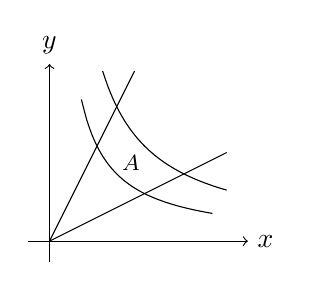
\begin{tikzpicture}[scale=0.9]
    \draw[->] (-0.3,0) -- (2.8,0) node[right] {$x$};
    \draw[->] (0,-0.3) -- (0,2.5) node[above] {$y$};
    % Rette y = x/2 e y = 2x
    \draw (0,0) -- (2.5,1.25);
    \draw (0,0) -- (1.2,2.4);
    % Iperboli y = 1/x e y = 2/x
    \draw[domain=0.45:2.3, smooth] plot (\x, {0.9/\x});
    \draw[domain=0.75:2.5, smooth] plot (\x, {1.8/\x});
    \node at (1.15,1.1) {\footnotesize $A$};
\end{tikzpicture}
\end{center}
\pencilnote{(noto che non è normale)}
\[
\implies A = \left\{ (x, y) \in \mathbb{R}^2 : \frac{1}{2} \le \underbrace{\frac{y}{x}}_{v} \le 2, \ 1 \le \underbrace{yx}_{u} \le 2, \ x > 0 \right\}
\]
\[
\implies A = \left\{ (u, v) \in \mathbb{R}^2 : 1 \le u \le 2, \ \frac{1}{2} \le v \le 2 \right\}
\]
\begin{center}
\begin{tikzpicture}[scale=0.9]
    \draw[->] (-0.3,0) -- (2.6,0) node[right] {$u$};
    \draw[->] (0,-0.3) -- (0,2.2) node[above] {$v$};
    \draw[thick] (0.8,0.45) rectangle (1.7,1.6);
    \draw[dotted] (0.8,0.45) -- (0.8,0) node[below] {\footnotesize $1$};
    \draw[dotted] (1.7,0.45) -- (1.7,0) node[below] {\footnotesize $2$};
    \node at (1.25,1.02) {\footnotesize $A$};
\end{tikzpicture}
\end{center}
\pencilnote{(sorge il problema del ``passaggio'' da $dx\, dy$ al ``$du\, dv$'')}
\[
\begin{cases}
\dfrac{y}{x} = v \\[6pt]
yx = u
\end{cases}
\iff
\begin{cases}
y = vx \\
x^2 v = u
\end{cases}
\iff
\begin{cases}
y = \sqrt{uv} \\[4pt]
x = \sqrt{\dfrac{u}{v}}
\end{cases}
\iff
\begin{cases}
y(u, v) = \sqrt{uv} \\[4pt]
x(u, v) = \sqrt{\dfrac{u}{v}}
\end{cases}
\]
Calcoliamo la \underline{matrice jacobiana}:
\[
\frac{\partial(x, y)}{\partial(u, v)} = \begin{pmatrix}
\dfrac{\partial x}{\partial u} & \dfrac{\partial x}{\partial v} \\[10pt]
\dfrac{\partial y}{\partial u} & \dfrac{\partial y}{\partial v}
\end{pmatrix} = \begin{pmatrix}
\dfrac{1}{2\sqrt{uv}} & -\dfrac{1}{2v}\sqrt{\dfrac{u}{v}} \\[10pt]
\dfrac{1}{2}\sqrt{\dfrac{v}{u}} & \dfrac{1}{2}\sqrt{\dfrac{u}{v}}
\end{pmatrix}
\]
Lo \underline{Jacobiano} è:
\[
\left| \det \frac{\partial(x, y)}{\partial(u, v)} \right| = \frac{1}{4v} + \frac{1}{4v} = \frac{1}{2v} \longrightarrow \text{al posto di } dx\, dy
\]
\[
\implies \iint_R \frac{1}{2} \frac{v}{v}\, du\, dv = \frac{1}{2} m(R) = \frac{1}{2} \left[ (2 - 1) \cdot \left(2 - \frac{1}{2}\right) \right] = \frac{3}{4}
\]
\pencilnote{($R$ rettangolo dato dal cambio)}
\end{esercizio}

\begin{definition}
Sia $D \subseteq \mathbb{R}^2$ normale, si dice \underline{regolare} se
\[
\left. \begin{cases}
\alpha(x), \beta(x) \text{ sono } C^1([a, b]) \text{ e} \\
\alpha(x) < \beta(x) \quad \forall x
\end{cases} \right\} \text{ se } D \text{ è norm. rispetto a } x
\]
oppure
\[
\left. \begin{cases}
\gamma(y), \delta(y) \text{ sono } C^1([c, d]) \text{ e} \\
\gamma(y) < \delta(y) \quad \forall y
\end{cases} \right\} \text{ se } D \text{ è norm. risp. a } y
\]
\end{definition}

\begin{definition}[Dominio regolare]
$D \subseteq \mathbb{R}^2$ si dice \underline{dominio regolare} se
\[
D = \bigcup_{i=1}^n D_i, \qquad \text{con } D_i \text{ normali regolari con } \mathring{D}_i \cap \mathring{D}_j = \emptyset \quad i \neq j
\]
\end{definition}

\begin{esercizio}[EXE]

\noindent\begin{minipage}{\linewidth}
\centering
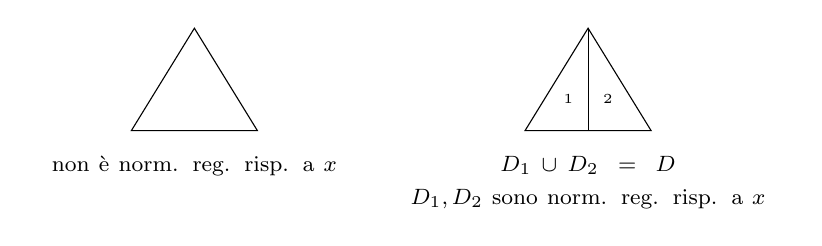
\begin{tikzpicture}
    % Triangolo non normale regolare
    \draw (0,0) -- (1.6,0) -- (0.8,1.3) -- cycle;
    \node[below, text width=4cm, align=center] at (0.8,-0.2)
        {\footnotesize non è norm. reg. risp. a $x$};

    \node at (3.3,0.65) {$\implies$};

    % Triangolo suddiviso in D1 e D2
    \begin{scope}[shift={(5,0)}]
        \draw (0,0) -- (1.6,0) -- (0.8,1.3) -- cycle;
        \draw (0.8,0) -- (0.8,1.3);
        \node at (0.55,0.4) {\tiny $1$};
        \node at (1.05,0.4) {\tiny $2$};
        \node[below, text width=5cm, align=center] at (0.8,-0.2)
            {\footnotesize $D_1 \cup D_2 = D$ \\ $D_1, D_2$ sono norm. reg. risp. a $x$};
    \end{scope}
\end{tikzpicture}
\end{minipage}

\medskip
% qui sotto il testo dell'esercizio
\end{esercizio}

Sia $T$ un dominio regolare e siano $(u, v)$ le sue coordinate.

Sia $\Phi : (u, v) \in T \to (x(u, v), y(u, v)) \in \mathbb{R}^2$, dove $x$ e $y$ sono $C^1(T)$ e sia $D = \Phi(T) \subseteq \mathbb{R}^2$ \pencilnote{(Immagine di $\Phi$, la prof l'ha chiamato immagine di $T$)}.

\begin{center}
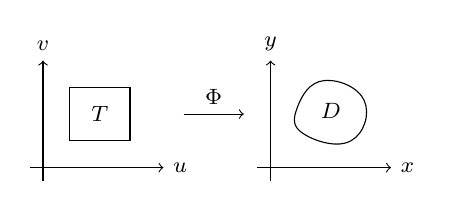
\begin{tikzpicture}[scale=0.85]
    % Piano (u, v)
    \begin{scope}[shift={(-2.2,0)}]
        \draw[->] (-0.2,0) -- (1.8,0) node[right] {\footnotesize $u$};
        \draw[->] (0,-0.2) -- (0,1.6) node[above] {\footnotesize $v$};
        \draw (0.4,0.4) rectangle (1.3,1.2);
        \node at (0.85,0.8) {\footnotesize $T$};
    \end{scope}
    \draw[->] (-0.1,0.8) -- (0.8,0.8) node[midway, above] {\footnotesize $\Phi$};
    % Piano (x, y)
    \begin{scope}[shift={(1.2,0)}]
        \draw[->] (-0.2,0) -- (1.8,0) node[right] {\footnotesize $x$};
        \draw[->] (0,-0.2) -- (0,1.6) node[above] {\footnotesize $y$};
        \draw plot [smooth cycle, tension=0.8] coordinates {(0.5,0.5) (1.2,0.4) (1.4,1.0) (0.8,1.3) (0.4,0.9)};
        \node at (0.9,0.85) {\footnotesize $D$};
    \end{scope}
\end{tikzpicture}
\end{center}

Poniamo
\[
\frac{\partial(x, y)}{\partial(u, v)} = \begin{pmatrix}
\dfrac{\partial x}{\partial u} & \dfrac{\partial x}{\partial v} \\[10pt]
\dfrac{\partial y}{\partial u} & \dfrac{\partial y}{\partial v}
\end{pmatrix} \qquad \text{che si chiama \underline{matrice jacobiana}.}
\]
Il suo determinante si chiama \underline{Jacobiano}. Allora vale il seguente teorema:

\begin{theorem}[Teo (s.d.)]
Siano $T, D \subseteq \mathbb{R}^2$ tali che $\exists \Phi : T \to D$ (entrambi regolari).

Sia $\Phi$ di classe $C^1$ come sopra e in più supponiamo che
\[
\left| \frac{\partial(x, y)}{\partial(u, v)} \right| \neq 0 \qquad (\implies \exists \Phi^{-1}).
\]
Allora se $f : D \to \mathbb{R}$ è continua, si ha:
\[
\boxed{\iint_{D = \Phi(T)} f(x, y)\, dx\, dy = \iint_T f(x(u, v), y(u, v)) \underbrace{\left| \frac{\partial(x, y)}{\partial(u, v)} \right|}_{\text{Jacobiano}} du\, dv}
\]
\end{theorem}

\begin{esercizio}[EXE 1]
\[
\iint_D \log\left(1 + (x + y)^4\right)(x - y)^2\, dx\, dy, \qquad D = \{ (x, y) : x \ge 0, \ 0 \le y \le 2 - x \}
\]
\end{esercizio}

\begin{esercizio}[EXE 2]
Calc. volume della sfera $+$ vol. cilindro $+$ vol. cono.
\end{esercizio}

\subsection{Coordinate polari}

\[
\begin{cases}
x = \rho \cos \theta \\
y = \rho \sin \theta
\end{cases}
\qquad \text{con } \rho > 0 \text{ e } \theta \in [0, 2\pi], \qquad \rho = \sqrt{x^2 + y^2}
\]
Lo \underline{Jacobiano} è:
\[
\left| \frac{\partial(x, y)}{\partial(\rho, \theta)} \right| = \rho \qquad \text{\pencilnote{(per exe)}}
\]

\begin{esercizio}[ES 1]
\[
\iint_D \frac{1}{1 + x^2 + y^2}\, dx\, dy, \qquad D = \{ (x, y) : 0 \le y \le \sqrt{3}\, x, \ 1 \le x^2 + y^2 \le 9 \}
\]
\pencilnote{($0 \le \dfrac{y}{x} \le \sqrt{3}$, \ $1 \le x^2 + y^2 \le 9$)}

\begin{center}
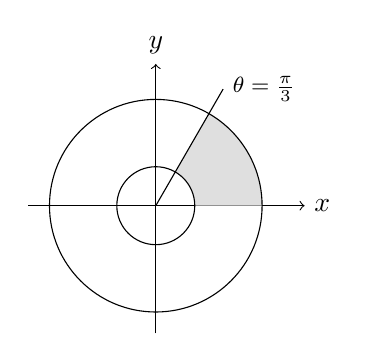
\begin{tikzpicture}[scale=0.9]
    \draw[->] (-1.8,0) -- (2.1,0) node[right] {$x$};
    \draw[->] (0,-1.8) -- (0,2.0) node[above] {$y$};
    \fill[gray!25] (0.55,0) -- (1.5,0) arc (0:60:1.5) -- (60:0.55) arc (60:0:0.55) -- cycle;
    \draw (0,0) circle (0.55);
    \draw (0,0) circle (1.5);
    \draw (0,0) -- (60:1.9) node[right] {\footnotesize $\theta = \frac{\pi}{3}$};
\end{tikzpicture}
\end{center}
\[
\begin{cases}
x = \rho \cos \theta \\
y = \rho \sin \theta
\end{cases}
\qquad \rho \in [1, 3], \quad \theta \in \left[0, \frac{\pi}{3}\right]
\]
\[
\implies R = \left\{ (\rho, \theta) : 0 \le \tan \theta \le \sqrt{3}, \ 1 \le \rho^2 \le 9 \right\}
\]
\[
= \iint_{[1, 3] \times \left[0, \frac{\pi}{3}\right]} \rho \frac{1}{1 + \rho^2}\, d\rho\, d\theta = \frac{\pi}{3} \int_1^3 \frac{\rho}{1 + \rho^2}\, d\rho
\]
\pencilnote{Se avessi avuto $D' = \{ 0 \le y - 1 \le \sqrt{3}\, x, \ 1 \le x^2 + (y - 1)^2 \le 9 \}$, avrei avuto $\begin{cases} x = \rho \cos \theta \\ y = \rho \sin \theta + 1 \end{cases}$.}
\end{esercizio}

\begin{esercizio}[EXE 2]
\[
\iint_D y(2 - x^2 - y^2)\, dx\, dy
\]
\[
D = \left\{ (x, y) : y \ge 0, \ (x - 1)^2 + y^2 \le 1, \ x^2 + y^2 \ge 2 \right\} \qquad \text{\pencilnote{Ho ''simmetria radiale'' rispetto a 2 centri}}
\]
\begin{center}
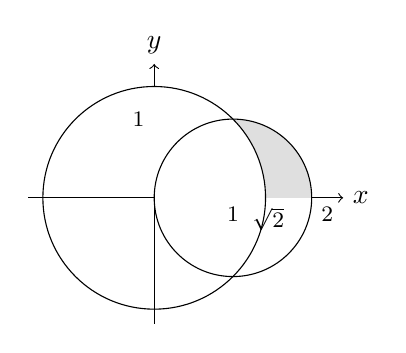
\begin{tikzpicture}[scale=1.0]
    \draw[->] (-1.6,0) -- (2.4,0) node[right] {$x$};
    \draw[->] (0,-1.6) -- (0,1.7) node[above] {$y$};
    % Regione D: y >= 0, (x-1)^2 + y^2 <= 1, x^2 + y^2 >= 2
    \begin{scope}
        \clip (0,0) rectangle (2.2,1.5);
        \fill[gray!25, even odd rule] (1,0) circle (1.0) (0,0) circle (1.414);
        \fill[white] (0,0) circle (1.414);
    \end{scope}
    \draw (0,0) circle (1.414);
    \draw (1,0) circle (1.0);
    \node[below] at (1,0) {\footnotesize $1$};
    \node[below] at (1.45,0) {\footnotesize $\sqrt{2}$};
    \node[below right] at (2,0) {\footnotesize $2$};
    \node[left] at (0,1) {\footnotesize $1$};
\end{tikzpicture}
\end{center}
\[
\begin{cases}
x = \rho \cos \theta \\
y = \rho \sin \theta
\end{cases}
\qquad \text{\pencilnote{(Scelgo il cambio di var. centrato nell'origine così che $\theta$ vari tra 2 estremi non entrambi le circ.)}}
\]
\[
\begin{cases}
x^2 + y^2 = 2 \\
(x - 1)^2 + y^2 = 1
\end{cases}
\iff
\begin{cases}
x^2 + y^2 = 2 \\
2 - 2x = 0
\end{cases}
\iff
\begin{cases}
y = 1 \\
x = 1
\end{cases}
\implies \theta \in \left[0, \frac{\pi}{4}\right]
\]
$\implies$ per trovare la ``dipendenza'' \pencilnote{dip. da $\theta$} nella parte ``esterna'', sostituisco le eq. in $D$:
\[
\rho^2 \ge 2 \implies \rho \ge \sqrt{2}, \qquad \rho^2 - 2\rho \cos \theta \le 0 \implies \rho \le 2 \cos \theta
\]
\[
\implies \rho \in [\sqrt{2}, 2 \cos \theta]
\]
\begin{align*}
&\implies \int_0^{\frac{\pi}{4}} \left[ \int_{\sqrt{2}}^{2 \cos \theta} \rho^2 \sin \theta (2 - \rho^2)\, d\rho \right] d\theta = \int_0^{\frac{\pi}{4}} \sin \theta \left[ \int_{\sqrt{2}}^{2 \cos \theta} (2\rho^2 - \rho^4)\, d\rho \right] d\theta = \\[6pt]
&= \int_0^{\frac{\pi}{4}} \sin \theta \left[ \frac{2}{3}\rho^3 - \frac{\rho^5}{5} \right]_{\sqrt{2}}^{2 \cos \theta} d\theta =
\end{align*}
\end{esercizio}



% 23-11.tex -- Formule di Gauss-Green, Teorema dei semplicemente connessi,
%             Teorema della divergenza, Solidi di rotazione e Integrali tripli (23/11/2026)

\subsection{Formule di Gauss--Green}

\begin{theorem}[Formule di Gauss--Green]
Sia $f : D \subseteq \mathbb{R}^2 \to \mathbb{R}$, $f \in C^1(D)$, dove $D$ è un \underline{dominio regolare}. Allora valgono le seguenti \underline{formule di Gauss--Green}:
\begin{enumerate}
    \item $\displaystyle \iint_D \frac{\partial f}{\partial x}\, dx\, dy = \oint_{+\partial D} f\, dy$
    \item $\displaystyle \iint_D \frac{\partial f}{\partial y}\, dx\, dy = -\oint_{+\partial D} f\, dx$
\end{enumerate}
\pencilnote{(Essendo integrali di linea, conta il verso di percorrenza: $+\partial D$ indica la frontiera orientata positivamente, cioè in senso antiorario.)}
\end{theorem}

\begin{proof}
Assumiamo inizialmente che $D$ sia \underline{normale regolare rispetto a entrambi gli assi}. Dimostriamo la (1) (la (2) si dimostra in modo analogo per esercizio).

Possiamo guardare $D$ come dominio normale rispetto a $y$:
\[
D = \{ (x, y) \in \mathbb{R}^2 : c \le y \le d, \ \gamma(y) \le x \le \delta(y) \}
\]
\begin{center}
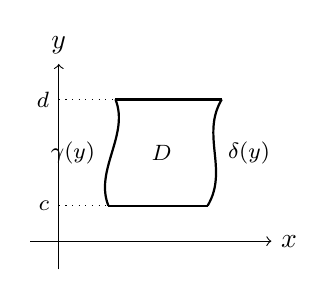
\begin{tikzpicture}[scale=0.9]
    \draw[->] (-0.4,0) -- (3.0,0) node[right] {$x$};
    \draw[->] (0,-0.4) -- (0,2.5) node[above] {$y$};
    \draw[thick] (0.7,0.5) -- (2.1,0.5);
    \draw[thick] (0.8,2.0) -- (2.3,2.0);
    \draw[thick] (0.7,0.5) .. controls (0.5,1.0) and (1.0,1.5) .. (0.8,2.0);
    \draw[thick] (2.1,0.5) .. controls (2.4,1.0) and (2.0,1.5) .. (2.3,2.0);
    \draw[dotted] (0,0.5) node[left] {\footnotesize $c$} -- (0.7,0.5);
    \draw[dotted] (0,2.0) node[left] {\footnotesize $d$} -- (0.8,2.0);
    \node[left] at (0.65,1.25) {\footnotesize $\gamma(y)$};
    \node[right] at (2.25,1.25) {\footnotesize $\delta(y)$};
    \node at (1.45,1.25) {\footnotesize $D$};
\end{tikzpicture}
\end{center}

Calcoliamo l'integrale doppio usando le formule di riduzione:
\[
\iint_D \frac{\partial f}{\partial x}(x, y)\, dx\, dy
= \int_c^d \left[ \int_{\gamma(y)}^{\delta(y)} \frac{\partial f}{\partial x}(x, y)\, dx \right] dy
= \underbrace{\int_c^d \big[ f(\delta(y), y) - f(\gamma(y), y) \big]\, dy}_{\text{I}}
\]

Ora calcoliamo $\displaystyle\oint_{+\partial D} f(x, y)\, dy$ parametrizzando $+\partial D = \gamma_1 \cup \gamma_2 \cup \gamma_3 \cup \gamma_4$:
\begin{center}
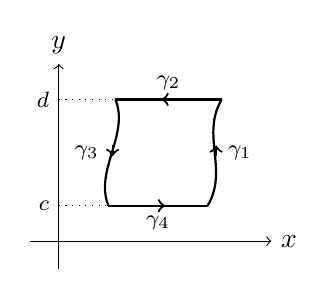
\begin{tikzpicture}[scale=0.9]
    \draw[->] (-0.4,0) -- (3.0,0) node[right] {$x$};
    \draw[->] (0,-0.4) -- (0,2.5) node[above] {$y$};
    \draw[thick] (0.7,0.5) -- (2.1,0.5);
    \draw[thick] (0.8,2.0) -- (2.3,2.0);
    \draw[thick] (0.7,0.5) .. controls (0.5,1.0) and (1.0,1.5) .. (0.8,2.0);
    \draw[thick] (2.1,0.5) .. controls (2.4,1.0) and (2.0,1.5) .. (2.3,2.0);
    \draw[->, thick] (1.35,0.5) -- (1.5,0.5);
    \draw[->, thick] (2.22,1.2) -- (2.22,1.35);
    \draw[->, thick] (1.6,2.0) -- (1.45,2.0);
    \draw[->, thick] (0.76,1.35) -- (0.76,1.2);
    \draw[dotted] (0,0.5) node[left] {\footnotesize $c$} -- (0.7,0.5);
    \draw[dotted] (0,2.0) node[left] {\footnotesize $d$} -- (0.8,2.0);
    \node[right] at (2.25,1.25) {\footnotesize $\gamma_1$};
    \node[above] at (1.55,2.0) {\footnotesize $\gamma_2$};
    \node[left] at (0.7,1.25) {\footnotesize $\gamma_3$};
    \node[below] at (1.4,0.5) {\footnotesize $\gamma_4$};
\end{tikzpicture}
\end{center}
\[
\oint_{+\partial D} f\, dy = \int_{\gamma_1} f\, dy + \int_{\gamma_2} f\, dy + \int_{\gamma_3} f\, dy + \int_{\gamma_4} f\, dy = *
\]
\begin{itemize}
    \item Su $\gamma_2$ e $\gamma_4$ la variabile $y$ è costante ($y = d$ e $y = c$), quindi $dy = 0$ e $\displaystyle\int_{\gamma_2} f\, dy = \int_{\gamma_4} f\, dy = 0$.
    \item Parametrizziamo $\gamma_1$ e $-\gamma_3$ (dal basso verso l'alto):
    \[
    \gamma_1 : \begin{cases} x = \delta(t) \\ y = t \end{cases} \quad t \in [c, d], \qquad
    -\gamma_3 : \begin{cases} x = \gamma(t) \\ y = t \end{cases} \quad t \in [c, d] \qquad (y'(t) = 1)
    \]
\end{itemize}
Sostituendo otteniamo:
\[
* = \int_{\gamma_1} f\, dy - \int_{-\gamma_3} f\, dy = \underbrace{\int_c^d \big[ f(\delta(t), t) - f(\gamma(t), t) \big]\, dt}_{\text{II}}
\]
Le espressioni I e II risultano uguali.

Nel caso generale, sia $D = \displaystyle\bigcup_{i=1}^N D_i$ con ciascun $D_i$ normale regolare rispetto a entrambi gli assi e $\mathring{D}_i \cap \mathring{D}_j = \emptyset$ per $i \neq j$. Allora:
\[
\iint_D \frac{\partial f}{\partial x}\, dx\, dy
= \sum_{i=1}^N \iint_{D_i} \frac{\partial f}{\partial x}\, dx\, dy
= \sum_{i=1}^N \oint_{+\partial D_i} f\, dy
= \oint_{+\partial D} f\, dy
\]
\begin{center}
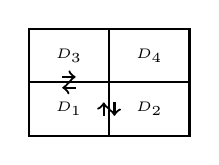
\begin{tikzpicture}[scale=0.85]
    \draw[thick] (0,0) rectangle (2.4,1.6);
    \draw[thick] (1.2,0) -- (1.2,1.6);
    \draw[thick] (0,0.8) -- (2.4,0.8);
    \draw[->, thick] (1.12,0.3) -- (1.12,0.5);
    \draw[->, thick] (1.28,0.5) -- (1.28,0.3);
    \draw[->, thick] (0.5,0.88) -- (0.7,0.88);
    \draw[->, thick] (0.7,0.72) -- (0.5,0.72);
    \node at (0.6,0.4) {\tiny $D_1$};
    \node at (1.8,0.4) {\tiny $D_2$};
    \node at (0.6,1.2) {\tiny $D_3$};
    \node at (1.8,1.2) {\tiny $D_4$};
\end{tikzpicture}
\end{center}
Infatti, lungo i tratti di bordo interni comuni a due domini adiacenti, la frontiera viene percorsa in entrambi i versi opposti e i rispettivi contributi si elidono; l'unico contributo che rimane è quello della frontiera esterna $+\partial D$.
\end{proof}

\begin{theorem}[Teorema dei semplicemente connessi]
\pencilnote{Teorema già citato nella lezione del 09-11, ma non dimostrato}
Sia $A \subseteq \mathbb{R}^2$ un aperto \underline{semplicemente connesso} e sia $\omega = a(x, y)\, dx + b(x, y)\, dy \in C^1(A)$.

Se $\omega$ è \underline{chiusa}, allora $\omega$ è \underline{esatta}.
\end{theorem}

\begin{proof}
Sia $\gamma$ una curva chiusa regolare e semplice con sostegno contenuto in $A$. Per il teorema di caratterizzazione delle forme esatte, basta dimostrare che $\displaystyle\oint_\gamma \omega = 0$.

Poiché $A$ è semplicemente connesso, la regione $D$ racchiusa da $\gamma$ è tutta contenuta in $A$ (ed è un dominio regolare con $\gamma = \pm\partial D$). Applicando le formule di Gauss--Green (a meno del verso di percorrenza di $\gamma$):
\begin{center}
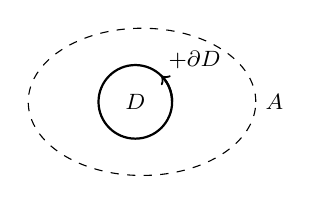
\begin{tikzpicture}[scale=0.85]
    \draw[dashed] (1.5,1.0) ellipse (1.7 and 1.1);
    \node[right] at (3.2,1.0) {\footnotesize $A$};
    \draw[thick] (1.4,1.0) circle (0.55);
    \draw[->, thick] (1.95,1.0) arc (0:45:0.55);
    \node at (1.4,1.0) {\footnotesize $D$};
    \node[above right] at (1.75,1.35) {\footnotesize $+\partial D$};
\end{tikzpicture}
\end{center}
\[
\pm \oint_\gamma \omega
= \oint_{+\partial D} a(x, y)\, dx + b(x, y)\, dy
= \iint_D \left( \frac{\partial b}{\partial x} - \frac{\partial a}{\partial y} \right) dx\, dy
= 0
\]
poiché $\omega$ è chiusa ($\dfrac{\partial b}{\partial x} = \dfrac{\partial a}{\partial y}$). Dunque $\displaystyle\oint_\gamma \omega = 0$ e $\omega$ è esatta.
\end{proof}

\begin{oss}
Nelle formule di Gauss--Green, scegliendo $f(x, y) = x$ (così $\dfrac{\partial f}{\partial x} = 1$) oppure $f(x, y) = y$ (così $\dfrac{\partial f}{\partial y} = 1$), si ottiene l'area di $D$ tramite un integrale curvilineo lungo la frontiera.
\end{oss}

\begin{theorem}[Area di un dominio regolare tramite la frontiera]
Sia $D \subseteq \mathbb{R}^2$ un dominio regolare. Allora:
\[
m(D) = \oint_{+\partial D} x\, dy = -\oint_{+\partial D} y\, dx = \frac{1}{2} \oint_{+\partial D} \left( -y\, dx + x\, dy \right)
\]
\end{theorem}

\begin{esercizio}[EXE -- Area dell'ellisse]
Calcolare l'area dell'ellisse $E = \left\{ (x, y) \in \mathbb{R}^2 : \dfrac{x^2}{a^2} + \dfrac{y^2}{b^2} \le 1 \right\}$ ($a, b > 0$).

\begin{center}
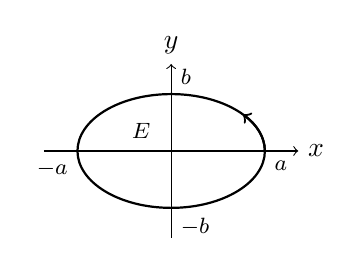
\begin{tikzpicture}[scale=0.85]
    \draw[->] (-1.9,0) -- (1.9,0) node[right] {$x$};
    \draw[->] (0,-1.3) -- (0,1.3) node[above] {$y$};
    \draw[thick] (0,0) ellipse (1.4 and 0.85);
    \draw[->, thick] (1.4,0) arc (0:40:1.4 and 0.85);
    \node[below right] at (1.4,0) {\footnotesize $a$};
    \node[below left] at (-1.4,0) {\footnotesize $-a$};
    \node[above right] at (0,0.85) {\footnotesize $b$};
    \node[below right] at (0,-0.85) {\footnotesize $-b$};
    \node at (-0.45,0.3) {\footnotesize $E$};
\end{tikzpicture}
\end{center}
Parametrizziamo $+\partial E$:
\[
+\partial E : \begin{cases} x = a \cos t \\ y = b \sin t \end{cases} \qquad t \in [0, 2\pi]
\]
Applicando la terza formula dell'area:
\[
A(E) = m(E) = \frac{1}{2} \int_0^{2\pi} \big( a b \sin^2 t + a b \cos^2 t \big)\, dt = \frac{1}{2} \int_0^{2\pi} ab\, dt = \pi a b
\]
\end{esercizio}

\subsection{Teorema della divergenza nel piano}

\begin{theorem}[Teorema della divergenza]
Sia $D \subseteq \mathbb{R}^2$ un dominio regolare e sia $F = (F_1, F_2)$ un campo vettoriale su $D$ di classe $C^1(D)$. Allora:
\[
\boxed{\iint_D \operatorname{div} F\, dx\, dy = \oint_{+\partial D} \langle F, N \rangle\, ds}
\]
dove:
\begin{itemize}
    \item $\operatorname{div} F = \dfrac{\partial F_1}{\partial x} + \dfrac{\partial F_2}{\partial y}$ è la \underline{divergenza} di $F$;
    \item $N$ è il \underline{versore normale esterno} a $\partial D$ (punta fuori da $D$), dato lungo una parametrizzazione antioraria $\gamma(t) = (x(t), y(t))$ da
    \[
    N(t) = \frac{(y'(t), -x'(t))}{\sqrt{x'(t)^2 + y'(t)^2}}
    \]
\end{itemize}
\end{theorem}

\begin{proof}
(Per esercizio obbligatorio, applicando le formule di Gauss--Green a $F_1$ e $F_2$).
\end{proof}

\subsection{Solidi di rotazione}

\begin{theorem}[$1^\circ$ Teorema di Guldino]
Sia $D \subseteq \mathbb{R}^2$ un dominio regolare e sia $r$ una retta complanare che non interseca la parte interna di $D$ \pencilnote{(al massimo può toccare il bordo)}. Sia $S$ il solido ottenuto ruotando $D$ intorno a $r$ di un angolo $\alpha \in (0, 2\pi]$.

Allora il volume di $S$ è dato dal prodotto dell'area di $D$ per la lunghezza dell'arco di circonferenza descritto dal suo \underline{baricentro} nella rotazione.
\end{theorem}

\begin{esercizio}[EXE -- Esempi notevoli]
Calcolare, mediante il $1^\circ$ teorema di Guldino, il volume dei seguenti solidi di rotazione: cilindro, tronco di cono, cono e toro.

\begin{center}
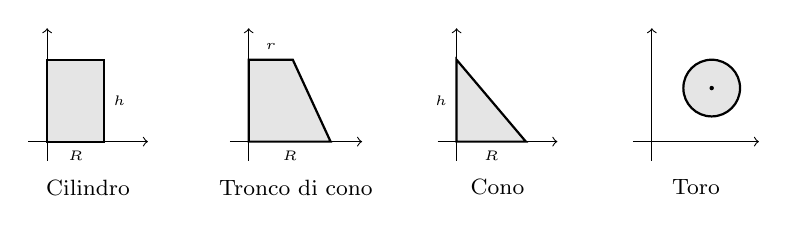
\begin{tikzpicture}[scale=0.8]
    % Cilindro
    \begin{scope}[shift={(-4.8,0)}]
        \draw[->] (-0.3,0) -- (1.6,0);
        \draw[->] (0,-0.3) -- (0,1.8);
        \fill[gray!20] (0,0) rectangle (0.9,1.3);
        \draw[thick] (0,0) rectangle (0.9,1.3);
        \node[below] at (0.45,0) {\tiny $R$};
        \node[right] at (0.9,0.65) {\tiny $h$};
        \node[below] at (0.65,-0.45) {\footnotesize Cilindro};
    \end{scope}
    % Tronco di cono
    \begin{scope}[shift={(-1.6,0)}]
        \draw[->] (-0.3,0) -- (1.8,0);
        \draw[->] (0,-0.3) -- (0,1.8);
        \fill[gray!20] (0,0) -- (1.3,0) -- (0.7,1.3) -- (0,1.3) -- cycle;
        \draw[thick] (0,0) -- (1.3,0) -- (0.7,1.3) -- (0,1.3) -- cycle;
        \node[below] at (0.65,0) {\tiny $R$};
        \node[above] at (0.35,1.3) {\tiny $r$};
        \node[below] at (0.75,-0.45) {\footnotesize Tronco di cono};
    \end{scope}
    % Cono
    \begin{scope}[shift={(1.7,0)}]
        \draw[->] (-0.3,0) -- (1.6,0);
        \draw[->] (0,-0.3) -- (0,1.8);
        \fill[gray!20] (0,0) -- (1.1,0) -- (0,1.3) -- cycle;
        \draw[thick] (0,0) -- (1.1,0) -- (0,1.3) -- cycle;
        \node[below] at (0.55,0) {\tiny $R$};
        \node[left] at (0,0.65) {\tiny $h$};
        \node[below] at (0.65,-0.45) {\footnotesize Cono};
    \end{scope}
    % Toro
    \begin{scope}[shift={(4.8,0)}]
        \draw[->] (-0.3,0) -- (1.7,0);
        \draw[->] (0,-0.3) -- (0,1.8);
        \fill[gray!20] (0.95,0.85) circle (0.45);
        \draw[thick] (0.95,0.85) circle (0.45);
        \fill (0.95,0.85) circle (1pt);
        \node[below] at (0.7,-0.45) {\footnotesize Toro};
    \end{scope}
\end{tikzpicture}
\end{center}
\end{esercizio}

\subsection{Integrali tripli}

\pencilnote{Prima della definizione di integrale triplo, occorre la definizione di dominio normale in $\mathbb{R}^3$.}

\begin{definition}[Dominio normale rispetto al piano $(x, y)$]
Un insieme $E \subseteq \mathbb{R}^3$ si dice \underline{normale rispetto al piano $(x, y)$} se
\[
E = \{ (x, y, z) \in \mathbb{R}^3 : (x, y) \in D \text{ dominio normale di } \mathbb{R}^2 \text{ e } \alpha(x, y) \le z \le \beta(x, y) \}
\]
con $\alpha, \beta : D \to \mathbb{R}$ continue e $\alpha(x, y) \le \beta(x, y)$ per ogni $(x, y) \in D$.

\begin{center}
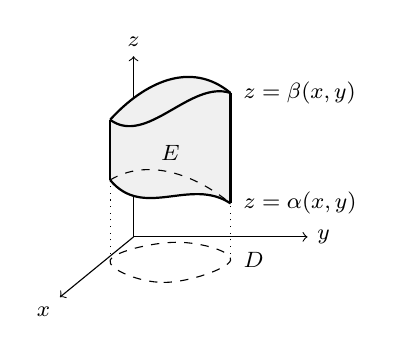
\begin{tikzpicture}[scale=0.85]
    \draw[->] (0,0) -- (2.6,0) node[right] {\footnotesize $y$};
    \draw[->] (0,0) -- (0,2.7) node[above] {\footnotesize $z$};
    \draw[->] (0,0) -- (-1.1,-0.9) node[below left] {\footnotesize $x$};

    % Proiezione D sul piano xy (dominio generico)
    \draw[dashed] plot[smooth cycle, tension=0.75] coordinates {
        (-0.35,-0.35) (0.45,-0.68) (1.45,-0.35) (0.65,-0.08)
    };
    \node[right] at (1.5,-0.35) {\footnotesize $D$};

    % Linee di proiezione verticale
    \draw[dotted] (-0.35,-0.35) -- (-0.35,0.85);
    \draw[dotted] (1.45,-0.35) -- (1.45,0.50);

    % Riempimento leggero del cilindroide E
    \fill[gray!12] (-0.35,0.85)
        .. controls (0.15,0.25) and (0.85,0.90) .. (1.45,0.50)
        -- (1.45,2.15)
        .. controls (0.85,2.65) and (0.15,2.30) .. (-0.35,1.75)
        -- cycle;

    % Superficie inferiore z = alpha(x, y) (inclinata e ondulata)
    \draw[thick] (-0.35,0.85) .. controls (0.15,0.25) and (0.85,0.90) .. (1.45,0.50);
    \draw[dashed] (-0.35,0.85) .. controls (0.20,1.18) and (0.90,0.95) .. (1.45,0.50);

    % Superficie superiore z = beta(x, y) (inclinata in senso opposto e ondulata)
    \draw[thick] (-0.35,1.75) .. controls (0.20,1.35) and (0.85,2.35) .. (1.45,2.15);
    \draw[thick] (-0.35,1.75) .. controls (0.15,2.30) and (0.85,2.65) .. (1.45,2.15);

    % Generatrici verticali laterali
    \draw[thick] (-0.35,0.85) -- (-0.35,1.75);
    \draw[thick] (1.45,0.50) -- (1.45,2.15);

    % Etichette
    \node at (0.55,1.25) {\footnotesize $E$};
    \node[right] at (1.5,2.15) {\footnotesize $z = \beta(x, y)$};
    \node[right] at (1.5,0.50) {\footnotesize $z = \alpha(x, y)$};
\end{tikzpicture}
\end{center}

Per definizione, il volume (misura) di $E$ è:
\[
m(E) = \iint_D \big[ \beta(x, y) - \alpha(x, y) \big]\, dx\, dy
\]
\end{definition}

\begin{definition}[Partizione in domini normali]
Sia $E \subseteq \mathbb{R}^3$ un dominio normale. La famiglia $\mathcal{P} = \{ E_1, E_2, \dots, E_n \}$ si dice \underline{partizione di $E$ in domini normali} se:
\begin{enumerate}
    \item $E_i \subseteq \mathbb{R}^3$ è normale $\forall i = 1, \dots, n$;
    \item $\mathring{E}_i \cap \mathring{E}_j = \emptyset \quad \forall i \neq j$;
    \item $\displaystyle\bigcup_{i=1}^n E_i = E$.
\end{enumerate}
\end{definition}